\documentclass[a4paper]{article}
\usepackage{lab}

\begin{document}


\begin{titlepage}
\thispagestyle{fancy} %For the left header
\rhead{}
\chead{}
\lhead{ECGR XXXX-Section XXX}
\rfoot{}
\cfoot{}
\lfoot{}
\renewcommand{\headrulewidth}{0pt} %Removes horizontal line
    \begin{center}
        \vspace*{1cm}
        
      
       \Large\textbf{University of North Carolina at Charlotte \\[1pt]
	Department of Electrical and Computer Engineering} \\[2pt]
\textit{Laboratory Experiment Number\# Type Report Number Here} \\[5pt]
\textbf{Experiment One \\[5pt]
Experiment Two\\[5pt]
Experiment Three\\
}

\noindent\rule{15cm}{0.4pt}
\vfill
        \vspace{0.5cm}
        \textit{Laboratory Experiment Report\# X,X,X} \\
		Author: First, Last\\
		Lab Partner: First, Last	\\
		Date: "Enter Date" \\
        
        \vspace{1.5cm}
        
        
        
        \vfill
		\vfill
        
       \large This report was submitted in compliance with UNCC POLICY 407\\
THE CODE OF STUDENT ACADEMIC INTEGRITY, Revised November 6, 2014
(http://legal.uncc.edu/policies/up-407) \_\_. (Student’s Initials) 
        \vspace{0.8cm}
        
    

    \end{center}
\end{titlepage}


\section{Objectives}

\subsection{Experiment 1}
\lipsum[1]
\subsection{Experiment 2}
\lipsum[1]
\subsection{Experiment 1}
\lipsum[1]
\section{Equipment List}
\subsection{Experiment 1}
\begin{table}[H]
	\centering
	\caption{Equipment Used} %Change this to caption.
	%I generate my tables from 
	\label{EquipmentUsed}
	\begin{tabular}{|l||l|}
		\hline
		\textbf{Equipment Used}       & \textbf{Equipment Manufacturer}               \\
		\hline
		Equipment Used & Equipment Manuf                         \\
		\hline
		Wave Form Generator  & Equipment Manuf                       \\
		\hline
		Equipment Used         & Equipment Manuf \\
		\hline
	\end{tabular}
\end{table}
\subsection{Experiment 2}
\begin{table}[H]
	\centering
	\caption{Equipment Used} %Change this to caption.
	%I generate my tables from 
	\label{EquipmentUsed1}
	\begin{tabular}{|l||l|}
		\hline
		\textbf{Equipment Used}       & \textbf{Equipment Manufacturer}               \\
		\hline
		Equipment Used & Equipment Manuf                         \\
		\hline
		Wave Form Generator  & Equipment Manuf                       \\
		\hline
		Equipment Used         & Equipment Manuf \\
		\hline
	\end{tabular}
\end{table}
\subsection{Experiment 3}
\begin{table}[H]
	\centering
	\caption{Equipment Used} %Change this to caption.
	%I generate my tables from 
	\label{EquipmentUsed3}
	\begin{tabular}{|l||l|}
		\hline
		\textbf{Equipment Used}       & \textbf{Equipment Manufacturer}               \\
		\hline
		Equipment Used & Equipment Manuf                         \\
		\hline
		Wave Form Generator  & Equipment Manuf                       \\
		\hline
		Equipment Used         & Equipment Manuf \\
		\hline
	\end{tabular}
\end{table}
\section{Relevant Theory/Background Information}

\subsection{Experiment 1}
\lipsum[1]
Figure \ref{fig} is an example of a figure.
\begin{figure}[H]\label{fig}
	\begin{center}
		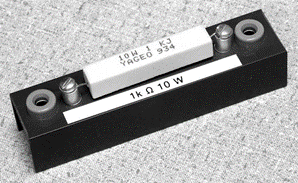
\includegraphics[width=6cm]{fig}
	\end{center}
	\caption{Example of a figure}
\end{figure}
\subsection{Experiment 2}
\lipsum[1]
\subsection{Experiment 3}
\lipsum[1]
\section{Experimental Data/Analysis}

\subsection{Experiment 1}
\lipsum[1]
\subsection{Experiment 2}
\lipsum[1]
\subsection{Experiment 3}
\lipsum[1]

\section{Conclusions}

\subsection{Experiment 1}
\lipsum[1]

\subsection{Experiment 2}
\lipsum[1]

\subsection{Experiment 3}
\lipsum[1]

\section{List of Attachments}
\listoffigures
\listoftables
\end{document}
